\section{Music to Our Ears: Standing Waves in Strings}

Name \rule{2.0in}{0.1pt}\hfill{}Section \rule{1.0in}{0.1pt}\hfill{}Date
\rule{1.0in}{0.1pt}

\textbf{Aim:}
\begin{itemize}
\item  to study the natural modes of vibration of a stretched string
\end{itemize}

\textbf{Equipment:}
\begin{itemize}
\item  string vibrator and power supply
\item  inelastic braided string
\item  2 clamps
\item  superpulley
\item  mounting rod for the superpulley
\item  mass and hanger set
\item  balance
\item  tape measure
\end{itemize}


How do we make musical sounds? To make a sound , we need something that vibrates. If we want to make musical notes you usually need the vibration to
have an almost constant frequency: that means stable pitch. We also want a frequency that can be easily controlled by the player. In electronic
instruments this is done with electric circuits or with clocks and memories. In non-electronic instruments, the stable, controlled vibration is
produced by a standing wave. Here we discuss the way strings work. This is also a good introduction for studying wind instruments, because vibrating
strings are easier to visualise than the vibration of the air in wind instruments, but the math is very similar.

\textbf{Introduction}

Waves are oscillations in an elastic medium:

\begin{itemize}
\item  your own vocal cords (the medium) vibrating as air is forced over them by your lungs; 
\item  a stretched string (the medium) on a musical instrument vibrating as it is bowed, hammered or plucked; 
\item  pressure oscillations in a column of air (the medium) in a wind instrument, organ pipe or your own oral and nasal cavities.
\end{itemize}

In each case the medium has an equilibrium state, and when displaced or otherwise perturbed from that state, experiences a force which tends to
restore it to equilibrium. For small perturbations, the restoring force is proportional to the displacement and the medium becomes a simple harmonic
oscillator.

There are also waves that do not require a medium, namely electromagnetic waves, which will be discussed later in the course.

\textbf{Background}

Standing waves (stationary waves) are produced by the interference of two traveling waves, both of which have the
same wavelength, speed and amplitude, but travel in opposite directions through the same medium. The necessary conditions for the production of
standing waves can be met in the case of a stretched string by having waves set up by some vibrating body, reflected at the end of the string and
then interfering with the oncoming waves.

One characteristic of every standing wave pattern is that there are points along the medium which appear to be standing still. These points,
sometimes described as points of no displacement, are referred to as nodes. There are other points along the medium which undergo vibrations between
a large positive and large negative displacement. These are the points which undergo the maximum displacement during each vibrational cycle of the
standing wave. In a sense, these points are the opposite of nodes, and so they are called antinodes. A standing wave pattern always consists of an
alternating pattern of nodes and antinodes. When a standing wave pattern is established in a medium, the nodes and the antinodes are always located
at the same position along the medium; they are "standing still." It is this characteristic which has earned the name "standing wave."

A stretched string has many natural modes of vibration (three examples are shown below). If the string is fixed at both ends then there must be a
node at each end. It may vibrate as a single segment, in which case the length ($L$) of the string is equal to 1/2 the wavelength ($\lambda $) of
the wave. It may also vibrate in two segments with a node at each end and one node in the middle; then the wavelength is equal to the length of the
string. It may also vibrate with a larger integer number of segments. In every case, the length of the string equals some integer number of half
wavelengths.

\vspace{0.3cm}
\begin{center}
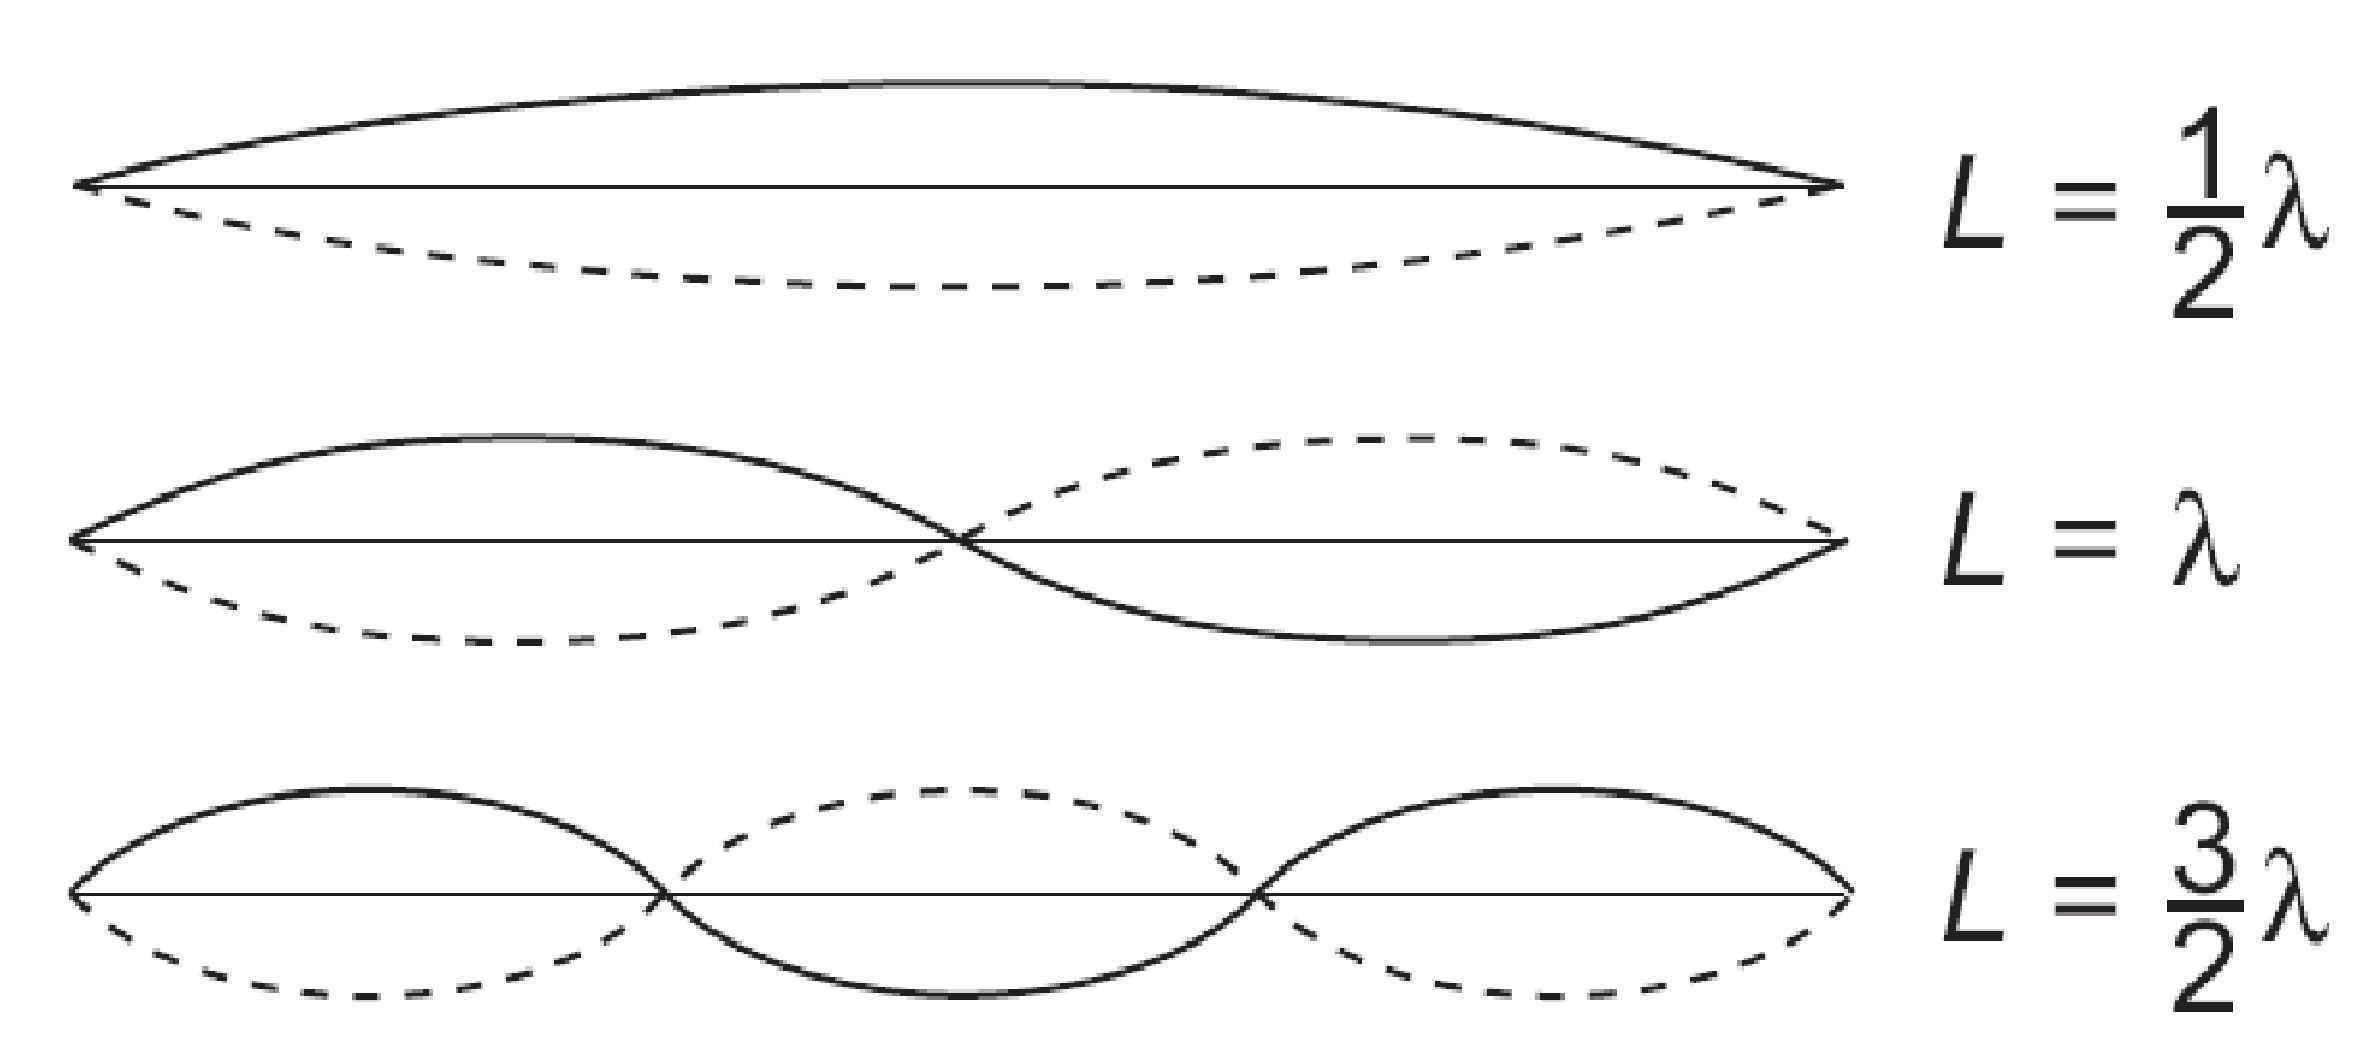
\includegraphics[width=3in]{standing_waves_strings/standing_waves_strings_fig1_tb.eps}
\end{center}
\vspace{0.3cm}

If you drive a stretched string at an arbitrary frequency, you will probably not see any particular mode; many modes will be mixed together. But, if
the tension and the string's length are correctly adjusted to the frequency of the driving vibrator, one vibrational mode will occur at a much
greater amplitude than the other modes.
For any wave with wavelength ($\lambda $) and frequency $f$, the speed, $v$, is:
\begin{equation}
v=\lambda f
\end{equation}

The speed of a wave on a string is also given by:
\begin{equation}
v=\sqrt{\frac {T}{\mu }}
\end{equation}
where $T$ is the tension in the string and $\mu $ is the linear density (mass/length) of the string.

In this experiment, standing waves are set up in a stretched string by the vibrations of an electrically-driven String Vibrator. The tension in the
string equals the weight of the masses suspended over the pulley. You can alter the tension by
changing the masses. $L$ is the length of the string and $n$ is the number of segments. (Note that $n$ is not the number of nodes). Since a segment
is 1/2 wavelength then


\begin{equation}
\lambda =\frac {2L}{n } \qquad n=1,2,3,...
\end{equation}



\vspace{0.3cm}
\begin{center}
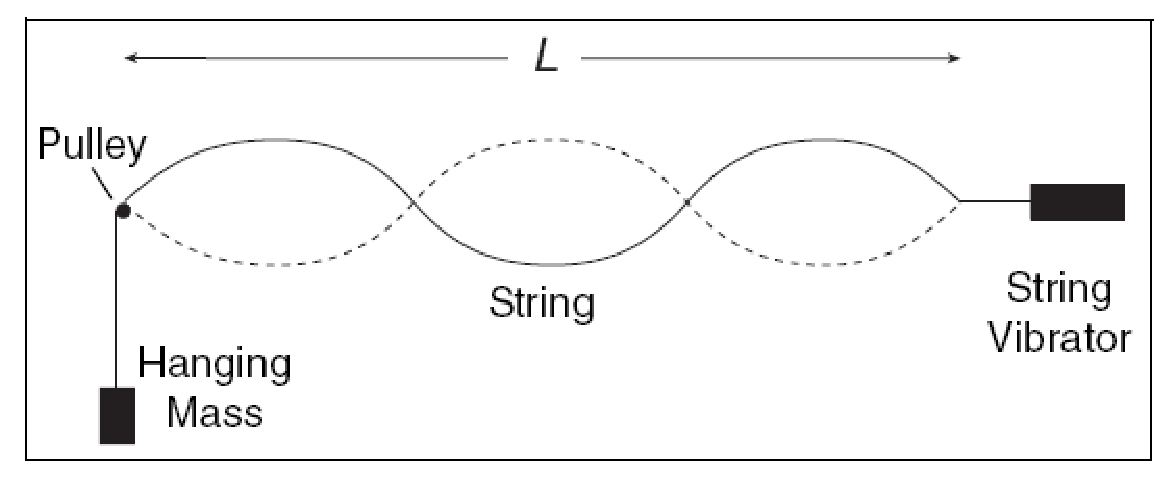
\includegraphics[width=250pt]{standing_waves_strings/standing_waves_strings_figure2.eps}
%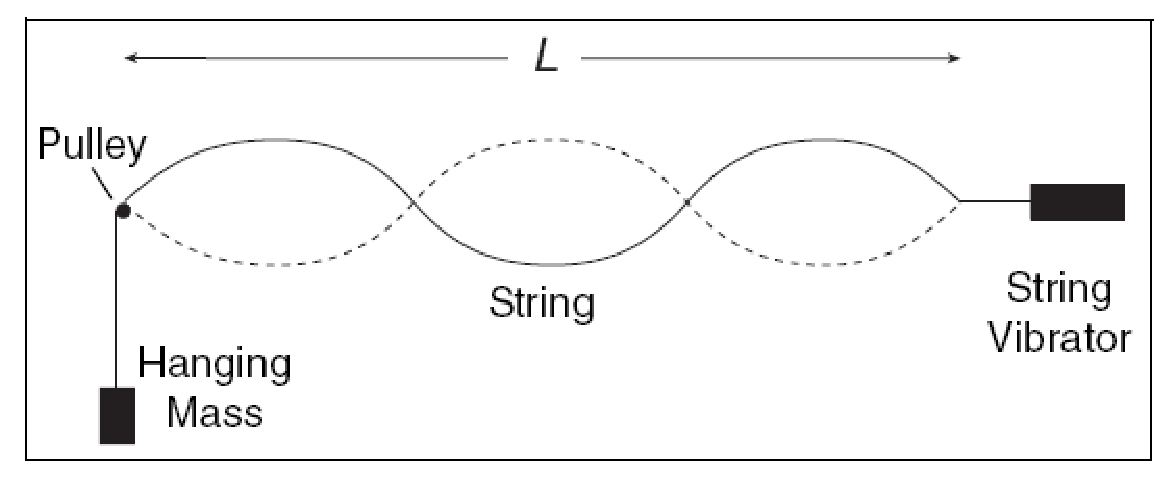
\includegraphics[width=3in]{standing_waves_strings/standing_waves_strings_figure2.eps}
\end{center}
\vspace{0.3cm}


\textbf{Procedure}

\textbf{1. } Measure the exact length of a piece of string several meters long. Measure the mass of the
string and calculate the linear density (mass/length).(If your balance is not precise enough to measure that length of string, use a longer
piece of string to calculate the linear density.)

\vspace{2cm}

\textbf{2. } Clamp the String Vibrator and pulley about 100 cm apart. Attach the string to the vibrating blade, run it over the pulley, and hang
about 200 g of mass from it. Cut off the excess string.

\textbf{3. } Measure from the knot where the string attaches to the String Vibrator to the top of the pulley.
This is the distance $L$. ($L$ is NOT the total length of the string that you measured in \textbf{1 }.) Record the value here: $L$ =

\vspace{0.3cm}
\begin{center}
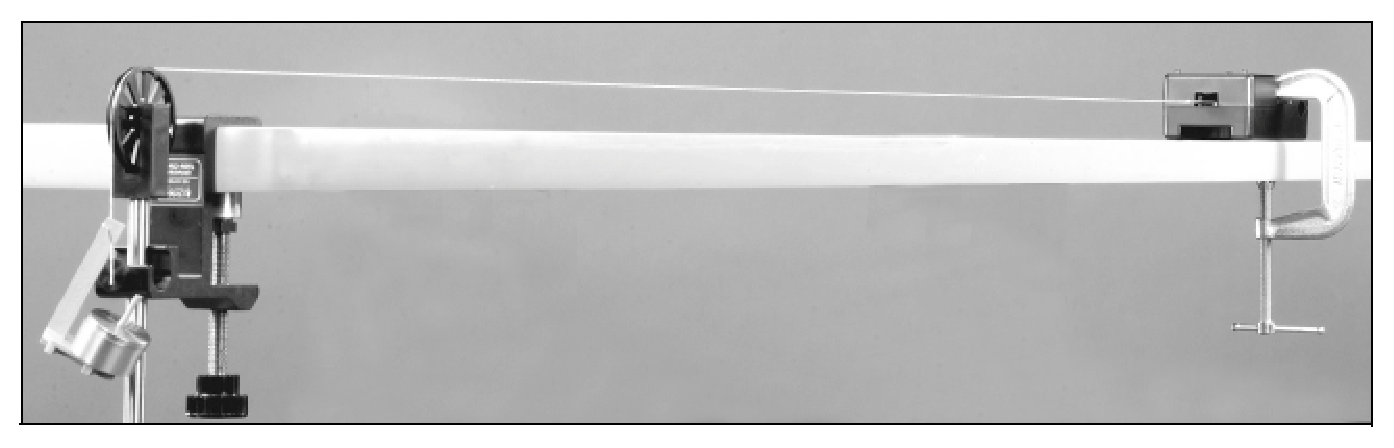
\includegraphics[width=320pt]{standing_waves_strings/standing_waves_strings_figure3.eps}
\end{center}
\vspace{0.3cm}

\textbf{4. } Connect the AC power supply to the String Vibrator.

\textbf{5. } Adjust the tension by adding to or subtracting from the hanging mass so that the string vibrates in 2 segments. Adjust the tension
further to achieve a ``clean'' node at the center. Also check the end of the vibrating blade; the point where the string attaches should be a node.
It is more important to have a good node at the blade than it is to have the largest amplitude possible. However, it is desirable to have the
largest amplitude possible while keeping a good node.

\textbf{6. } Record the hanging mass, $m$. How much uncertainty is there in your value? By how much can you change the hanging mass before you see
an effect? Record the uncertainty.

\vspace{3cm}

\textbf{Part A: Speed of the Wave }

\textbf{a. } Calculate the tension (including the uncertainty) in the string.

\vspace{3cm}

\newpage

\textbf{b. } Calculate the speed $v_A$ (including uncertainty) of the wave from your observed values of tension
($T$) and linear density ($\mu $). Record your calculated value with the uncertainty and the correct number of significant
figures.


\vspace{4cm}

\textbf{c. } Calculate the speed $v_B$ from the wavelength ($\lambda $) and frequency ($f$). (In the U.S. $f$ = 60.0 Hz.)

\vspace{4cm}

\textbf{d. } Compare the two values ($v_A$ and $v_B$) of speed. What is the difference? How does the difference compare
to the uncertainty that you determined in \textbf{b }?

\vspace{4cm}

\textbf{e. } Calculate the percentage by which $v_A$ deviates from $v_B$.

\begin{equation}
\% Deviation =\frac {v_A - v_B}{v_B} \times 100\%
\end{equation}

\vspace{3cm}

\newpage

\textbf{Part B: Linear Density}

\textbf{a. } Produce standing waves of 3, 4, 5, etc. segments in the string by reducing the hanging mass. Get as many as you can. Create a table
here with the headings $n$ (number of segments), $m$ (mass), $T$ (tension in the string which is the same as $mg$), and $\frac{1}{n^2}$. Be sure to
include the result from Part A for n = 2.

\vspace{6cm}

\textbf{b. } For every value of mass, calculate the tension in the string, and include in the above table.

\textbf{c. } In $Excel$, plot a graph of $T$ versus $n$ including a trend line 
using a power function. Print the graph and include it with this unit. What is 
the power of $n$?
\vspace{20mm}

\textbf{d. } For every value of $n$, calculate $\frac{1}{n^2}$ and include in above table. In $Excel$, plot a graph of $T$ versus $\frac{1}{n^2}$.
Does the graph look linear? If so, include a linear trend line. Print the graph and include it with this unit.
\vspace{20mm}

\textbf{e. } Using the LINEST function in $Excel$ (see \textbf{Appendix C}), find the slope of the graph and its uncertainty. Record the values here
(including units):

\vspace{20mm}

\textbf{f. } Combine the equations in the \textbf{Background } section, and show that the tension can be written as:

\begin{equation}
T=4\mu f^{2}L^{2}\frac{1}{n^2}
\end{equation}

\vspace{25mm}

Thus the slope of a $T$ versus $\frac{1}{n^2}$ graph is $4\mu f^{2}L^{2}$.

\textbf{g. } Use the slope from your graph to calculate the density, $\mu $, of the string. Also calculate the uncertainty in $\mu$, assuming the
fractional uncertainty in $\mu$ is the same as the fractional uncertainty in the slope.

\vspace{5cm}

\textbf{h. } Compare this measured value of string density to the accepted value. (You calculated the accepted value of $\mu $ from the mass and
length of the string at the beginning of the experiment). Does the accepted value fall within the uncertainty limits of your calculated value?

\vspace{50mm}

%\textbf{i. } Calculate the percent deviation of the measured value of $\mu $ from the accepted value.

%\begin{equation}
%\% Deviation =\frac{Measured-Accepted}{Accepted}\times 100\%
%\end{equation}

%\vspace{4cm}

\textbf{Further Investigation}

%\textbf{1. } Hang a mass on the string with a value that is about halfway between the masses that produced standing waves of 3 and 4 segments. The
string should show no particular mode. Place a ``bridge'' so that you can see the exact fundamental ($n = 1$) between the String
%Vibrator and the bridge. What is the wavelength?

%\vspace{1.5cm}

%Slide the bridge away from String Vibrator until the string vibrates in 2 segments. How does the wavelength of the two-segment wave compare to the
wavelength of the previous one segment wave?

%\vspace{1.5cm}

%Why is a standing wave created only when the bridge is at certain locations? What are these locations called?

%\vspace{1.5cm}

If a strobe is available, observe the standing wave on a string with the 
strobe light. Draw a diagram explaining the motion of the string.




